\documentclass[a4paper,11pt]{article}
\usepackage[utf8]{inputenc}
\usepackage[T1]{fontenc}
\usepackage[french]{babel}
\usepackage{makeidx}
\usepackage{textcomp}
\usepackage{graphicx}
\usepackage{mathtools,amssymb,amsthm}
\usepackage{lmodern}
\usepackage{multirow}
\usepackage{listings}
\usepackage{array}
\usepackage{longtable}

\title{Projet simulation - Rapport}
\author{Maxime Gonthier (21500231) - Benjamin Guillot (21500545)}

\begin{document}
\pagenumbering{gobble}\clearpage
\maketitle

\newpage
\tableofcontents

\newpage
\section{Introduction}
	L'objectif de ce projet est de simuler en temps discret des arrivées et des services dans un cyber café. On en déduira des mesures d'évaluations à l'aide du calcul du temps moyen d'attente et du 90ème percentile du temps d'attente. 
\newpage
\section{Explication de la programmation}
	\subsection{Entrée et sortie du progamme}
	En entrée le programme prend un fichier texte contenant les données que l'on veut faire varier dans notre application (ici lambda).
	On obtient en sortie 5 fichier :
	\begin{itemize}
		\item Result\_modele1.txt
		\item Result\_modele2.txt
		\item Result\_modele3.txt
		\item resultE.txt
		\item result90.txt
	\end{itemize}
	Les 3 premiers fichiers contiennent pour chaque valeurs de lambda le temps moyen d'attente $E[A]$ et le 90 percentile du temps d'attente $t_{90}E[A]$.\\
	Les deux derniers fichiers sont utilisés pour l'affichages des courbes obtenues après la simulation.
	\subsection{structure du progamme}
	Nous avons choisit pour la programmation de gérés les différents modèles dans les fonctions $Arrivee\_Client$ et $service\_event$. Ces deux fonctions on 3 modes de fonctionnement
	passé en argument pour savoir quel modèle on est en train de simuler. Il y a un simulateur par modèles.
	Il sont appelés dans le main avec en argument :
	\begin{itemize}
		\item un fichier dans lequel écrire les données relatives a la simulation.
		\item la valeur de lambda en train d'être testée.
	\end{itemize}
	\subsubsection{premier modèle}
		le premier modèle représente une M/M/N classique. on traite donc les clients dès qu'un serveur est libre.
	\subsubsection{second modèle}
		Le second modèle peut être simulé avec une M/M/1. On ajoute une condition aux arrivées de client qui est un pourcentage de chance d'arriver dans la file, comme on a 10 serveurs en theorie, un client arrive dans une file avec une probabilité $\frac{1}{10}$.
	\subsubsection{troisième modèle}
		Le troisième modèle est simulé avec 10 M/M/1. On stocke dans un tableau le nombre de client par file et a chaque arrivée de client, on vérifie quelle est la file la moins rempli. Le client est envoyé sur cette file. On stocke dans l'évènement la file sur laquelle se trouve le client afin de pouvoir décrémenter le nombre de client de cette file après un service. 
	
\section{Analyse des résultats}
	Avant tout de chose, notons que pour le modèle 2, les valeurs que nous avons obtenus pour le temps moyen d'attente
	correspondent à 1/10 des clients d'une M/M/1. Ce qui revient au final à créer 10 M/M/1. Nous avons choisis cette ordre de grandeur
	plus petit pour pouvoir dessiner les 3 courbes sur le même graphe sans avoir à déformer énormément l'echelle. En effet sinon nous aurions dû 
	multiplier par 10 toutes les valeurs du temps moyen d'attente pour le modèle 2.\\
	\centerline{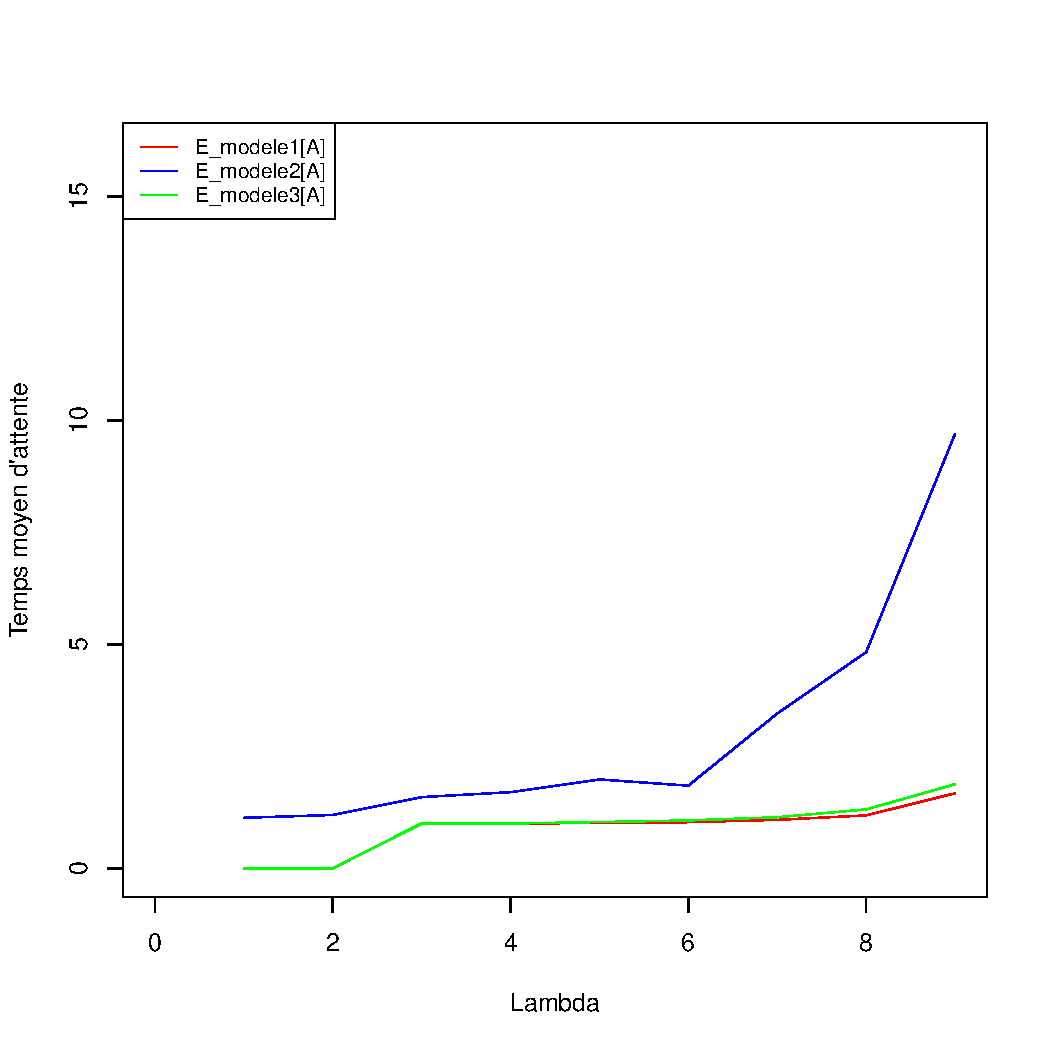
\includegraphics[scale=0.8]{E[A].pdf}}\\
	On observe que le temps moyen d'attente du modèle 2 augmente significativement à partir de lambda = 6. En effet il passe de moins de 3 à lambda = 6 à plus de 5 à lambda = 8.
	Cela s'explique par la manière dont se calcule le temps moyen d'attente dans une M/M/1. En effet on fait : \\
		$E[A] = \rho * \frac{\frac{1}{\mu}}{1-\rho}$\\
		avec : $\rho = \frac{\lambda}{\mu}$\\
		Donc plus lambda augmente, plus la valeur de rho est grande est donc plus le temps moyen d'attente est grand.
		En effet la multiplication par rho augmente plus la valeurs de E[A] que la division car rho > 1 - rho.
		A condition bien evidemment que ${\mu}$ ne soit pas trop élèvé, ce qui rendrait toute les valeurs de E[A] quasiments similaires à cause du ${\frac{1}{\mu}}$
	
	On observe que les modèles 1 et 3 ont des valeurs similaires de temps moyen d'attente. Cela s'explique par la similarité de leurs fonctionnement. En effet le modèle 1
	il y a une file avec 10 serveurs et dès qu'un serveur est libre on fais un service. Dans le 3 il y a 10 files et les clients vont dans la file la plus vide. Ainsi 
	dans les deux cas les clients sont servis dès qu'une place est libéré, que ce soit un serveur ou une file qui se libère. Cela explique bien la ressemblance des deux courbes. 
	Nous notons aussi que les temps moyen d'attente sont plus faibles pour le modèle 1 et 3 que pour le modèle 2. Cela vient du fait que le patron choisit aléatoirement un ordinateur, cela peut donc 
	de temps en temps ralentir le service car un client sera mis sur un ordinateur ou il y a déjà des clients qui attendent. Et donc cela augmentera le temps moyen d'attente de manière
	significative pour un grand nombre de clients.
	\newpage
	Le graphique des 90ème percentiles : \\
	\centerline{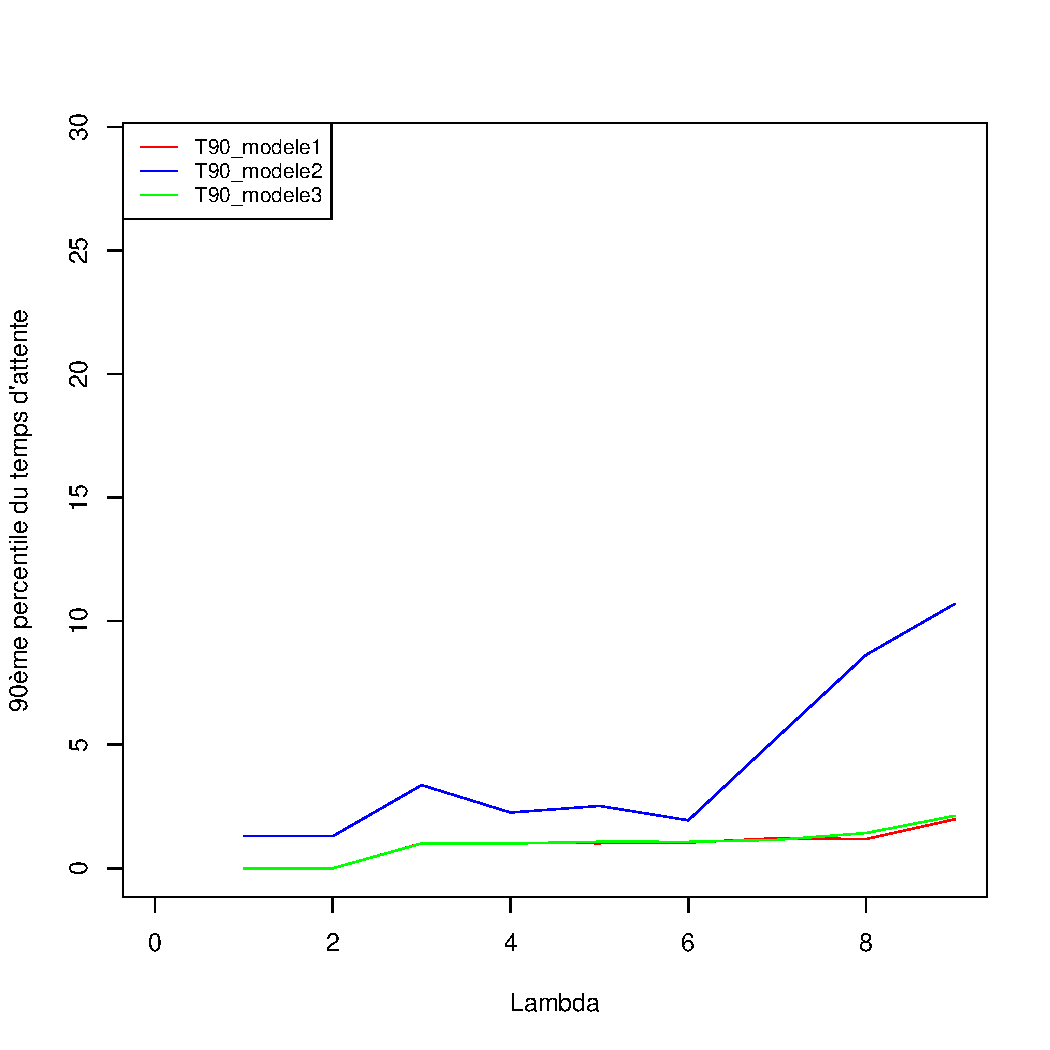
\includegraphics[scale=0.8]{t90.pdf}}\\
	
	On observe les mêmes résultats que pour le graphique précedent à l'exception de ce sursaut pour le modèle 2 à lambda = 3. 
	Cela s'explique par une "malchance" qui a fais que plusieurs clients ont été 
	mis sur des files dont le temps d'attente fût long comme expliqué au dessus, ce qui a donc augmenter le nombre de valeurs extrèmes dans le temps d'attente des clients. Or le 90 ème percentile
	prend la valeur dont 90\% des valeurs sont inférieures, donc si 10\% des valeurs des temps d'attente sont extrèmes, alors le 90ème percentile le sera aussi.

\section{Explication des résultats théoriques}
	
\section{Conclusion}
	Pour ce projet, nous aurions pu simplifier le code en utilisant un seul simulateur pour les 3 modèles, en ayant plusieurs cas d'usage. Nous aurions également pu découper le code en plus de fonctions afin de rendre celles-ci plus courtes et plus facilement compréhensible.
\end{document}
